\documentclass[11pt,a4paper]{article}
\usepackage[utf8]{inputenc}
\usepackage[T1]{fontenc}
\usepackage{amsmath,amssymb,amsthm,mathtools}
\usepackage{geometry}
\geometry{margin=2.5cm}
\usepackage{booktabs}
\usepackage{xcolor}
\usepackage{enumitem}
\usepackage{array}
\usepackage{lmodern}
\usepackage{microtype}
\usepackage{tikz}
\usetikzlibrary{arrows.meta,positioning}
\usepackage{hyperref}
\hypersetup{
    colorlinks=true,
    linkcolor=blue!70!black,
    citecolor=red!70!black,
    urlcolor=blue!70!black,
    pdftitle={Unconditional Formalization of Von Koch's Chebyshev Psi-Theorem and Modular Three-Frequency Forward Closure in Lean 4},
    pdfauthor={Qamar Munawer}
}

\newtheorem{theorem}{Theorem}[section]
\newtheorem{lemma}[theorem]{Lemma}
\newtheorem{proposition}[theorem]{Proposition}
\newtheorem{corollary}[theorem]{Corollary}
\theoremstyle{definition}
\newtheorem{definition}[theorem]{Definition}
\newtheorem{remark}[theorem]{Remark}

\newcommand{\dee}{\mathrm{d}}
\newcommand{\Nset}{\mathbb{N}}
\newcommand{\Rset}{\mathbb{R}}
\newcommand{\Cfield}{\mathbb{C}}

\title{\textbf{Unconditional Formalization of Von Koch's Chebyshev $\psi$-Theorem\\
and Modular Three-Frequency Forward Closure in Lean~4}}

\author{\textbf{Qamar Munawer}\\[0.3em]
\small Brandenburg University of Technology Cottbus--Senftenberg, Cottbus, Germany}

\date{November 18, 2026}

\begin{document}
\linespread{1.15}\selectfont
\emergencystretch=2.5em

\maketitle

\begin{abstract}
Prior formalizations of prime-number criteria in Lean~4 addressed Littlewood's M\"obius/Mertens criterion and constructive Nyman--Beurling cotangent kernels separately. This paper records two substantial Lean~4 formalization components absent from all six previously published micro-papers: (1) an axiom-free formalization of Von Koch's classical forward theorem in both \texttt{Section7\_\allowbreak SpectralBridge.lean} ($636$ lines) and \texttt{MathlibPR\_\allowbreak LittlewoodMertens.lean} ($342$ lines), proving unconditionally that $\psi(x) - x = \mathcal{O}(x^{1/2 + \varepsilon})$ for all $\varepsilon > 0$ implies \texttt{\_root\_.\allowbreak RiemannHypothesis} via Mellin analytic continuation across four overlapping convex open regions and order-of-zero factoring via \texttt{AnalyticAt} (\texttt{vonKoch\_\allowbreak implies\_\allowbreak rh}, \texttt{RiemannHypothesis.\allowbreak of\_\allowbreak chebyshevPsi\_\allowbreak sub\_\allowbreak self\_\allowbreak isBigO}); and (2) the complete five-stage conditional forward spectral closure architecture comprising \texttt{MathlibPR\_\allowbreak LinearMomentLimit.lean} ($195$ lines), \texttt{MathlibPR\_\allowbreak SpectralTailBound.lean} ($233$ lines), \texttt{MathlibPR\_\allowbreak MontgomeryVaughan.lean} ($279$ lines), \texttt{MathlibPR\_\allowbreak SelbergSieveBound.lean} ($215$ lines), and \texttt{MathlibPR\_\allowbreak ForwardClosure.lean} ($237$ lines). Across all modules ($1{,}795$ lines excluding the previously covered Mertens fragment), every theorem compiles cleanly with zero \texttt{sorry} placeholders and depends strictly on \texttt{[propext, Classical.choice, Quot.sound]}. Under \texttt{NO\_RH\_PROOF = TRUE}, the three-frequency closure theorems formalize exact machine-checked interfaces rather than asserting analytic proof of the constituent spectral hypotheses.
\end{abstract}

\noindent\textbf{Keywords:} Von Koch theorem, Chebyshev $\psi$ function, Mellin transform, Montgomery--Vaughan mean value, Selberg sieve majorant, forward Nyman--Beurling closure, Lean~4, Mathlib4.

\section{Introduction and Epistemic Scope}

Helge von Koch (1901) established that the prime-number remainder bound $\psi(x) - x = \mathcal{O}(x^{1/2}\ln^2 x)$ is closely tied to the Riemann Hypothesis; its $\varepsilon$-weakened equivalence $\psi(x) - x = \mathcal{O}(x^{1/2+\varepsilon})$ ($\forall \varepsilon > 0$) mirrors Littlewood's Mertens bound on the additive-logarithmic side of the zeta function via $-\zeta'(s)/\zeta(s)$. While Littlewood's M\"obius equivalence was formalized in earlier work, the Chebyshev $\psi(x)$ / Von Koch forward theorem in \texttt{Section7\_\allowbreak SpectralBridge.lean} and the modular five-stage forward closure pipeline (\texttt{MathlibPR\_\allowbreak LinearMomentLimit.lean} through \texttt{MathlibPR\_\allowbreak ForwardClosure.lean}) remained unrepresented in the published micro-paper series.

\paragraph{Epistemic Demarcation (\texttt{NO\_RH\_PROOF = TRUE}).}
Both components below operate strictly within the machine-checked standard axiom set \texttt{[propext, Classical.choice, Quot.sound]}:
\begin{itemize}[noitemsep]
  \item In Part~\ref{sec:vonkoch}, the implication \texttt{VonKochRemainderBound $\to$ \_root\_.\allowbreak RiemannHypothesis} is proved \emph{unconditionally}, whereas the converse direction $\mathrm{RH} \to \mathrm{VonKochRemainderBound}$ in \texttt{spectral\_\allowbreak stability\_\allowbreak theorem} remains explicitly isolated behind the analytical record \texttt{ClassicalAnalyticInterface} (reflecting truncated Perron contour integration not yet available in Mathlib4).
  \item In Part~\ref{sec:five_stage}, the linear cross-term identities and resolvent decay inequalities are unconditional, while the analytic bounds inside \texttt{LowFrequencyBound}, \texttt{MidFrequencyBound}, \texttt{FullSpectralSystem}, and \texttt{ForwardPillarSynthesis} are explicit structured interfaces whose discharge implies RH via \texttt{forward\_\allowbreak closure\_\allowbreak riemann\_\allowbreak hypothesis}.
\end{itemize}

\section{Unconditional Lean~4 Proof of Von Koch's Forward Theorem}\label{sec:vonkoch}

Let $\psi(x) = \sum_{n \le x} \Lambda(n)$ (\texttt{chebyshevPsi x}) denote Chebyshev's second prime-counting function. In \texttt{Section7\_\allowbreak SpectralBridge.lean} (and mirrored in self-contained Mathlib style inside \texttt{MathlibPR\_\allowbreak LittlewoodMertens.lean}), define the truncated remainder and its Mellin transform:
\begin{equation}
R_\psi(x) \coloneqq \mathbf{1}_{(1,\infty)}(x)\,(\psi(x) - x), \qquad
M_\psi(s) \coloneqq s \int_0^\infty R_\psi(x)\, x^{-s-1}\,\dee x
\end{equation}
(\texttt{chebyshevPsiRemainder} and \texttt{mellinVonKochRemainder}). The proof of \texttt{vonKoch\_\allowbreak implies\_\allowbreak rh} executes in four clean stages.

\subsection{Stage A--B: Analytic Continuation of $M_\psi(s)$ on $\operatorname{Re}(s) > 1/2$}
Unconditionally, \texttt{sum\_\allowbreak vonMangoldt\_\allowbreak Icc\_\allowbreak le\_\allowbreak mul\_\allowbreak log} proves $\sum_{k=1}^n \Lambda(k) \le n \ln n$, while \texttt{chebyshevPsi\allowbreak Remainder\_\allowbreak isBigO\_\allowbreak atTop\_\allowbreak uncond} and \texttt{chebyshevPsi\allowbreak Remainder\_\allowbreak locally\allowbreak IntegrableOn} establish measurability and local integrability. Under the hypothesis \texttt{VonKoch\allowbreak RemainderBound} ($\forall \varepsilon > 0,\; \psi(x) - x = \mathcal{O}(x^{1/2+\varepsilon})$), \texttt{chebyshevPsi\allowbreak Remainder\_\allowbreak isBigO\_\allowbreak atTop\_\allowbreak of\_\allowbreak vonKoch} and dominated differentiation prove \texttt{mellin\allowbreak VonKoch\allowbreak Remainder\_\allowbreak differentiableAt} and \texttt{mellin\allowbreak VonKoch\allowbreak Remainder\_\allowbreak analyticOnNhd} throughout the open half-plane $\{s \in \Cfield : 1/2 < \operatorname{Re}(s)\}$.

On the convergent region $\operatorname{Re}(s) > 1$, integrating $-\zeta'(s)/\zeta(s) = \sum_{n=1}^\infty \Lambda(n) n^{-s}$ by parts against $x^{-s}$ gives \texttt{neg\_\allowbreak deriv\_\allowbreak riemannZeta\_\allowbreak div\_\allowbreak eq\_\allowbreak pole\_\allowbreak add\_\allowbreak mellinVonKochRemainder} and the cleared holomorphic identity
\begin{equation}\label{eq:cleared_log_deriv}
\zeta'(s) + \left(\frac{s}{s - 1} + M_\psi(s)\right)\zeta(s) = 0 \qquad (\operatorname{Re}(s) > 1),
\end{equation}
formalized as \texttt{zeta\_\allowbreak deriv\_\allowbreak cleared\_\allowbreak eq\_\allowbreak zero\_\allowbreak of\_\allowbreak one\_\allowbreak lt\_\allowbreak re}.

\subsection{Stage C: Four-Convex-Set Identity Continuation Around $s = 1$}
Because the punctured half-plane $\{s \in \Cfield : 1/2 < \operatorname{Re}(s) \land s \neq 1\}$ is non-convex, Lean's convex identity theorem is applied across four overlapping open convex subsets (upper half $\{1/2 < \operatorname{Re}(s),\; \operatorname{Im}(s) > 0\}$, lower half $\{1/2 < \operatorname{Re}(s),\; \operatorname{Im}(s) < 0\}$, left strip $\{1/2 < \operatorname{Re}(s) < 1\}$, and right half $\{\operatorname{Re}(s) > 1\}$) to establish \texttt{zeta\_\allowbreak deriv\_\allowbreak cleared\_\allowbreak eq\_\allowbreak zero\_\allowbreak of\_\allowbreak half\_\allowbreak lt\_\allowbreak re\_\allowbreak ne\_\allowbreak one}: identity~\eqref{eq:cleared_log_deriv} holds at every point $s$ with $\operatorname{Re}(s) > 1/2$ and $s \neq 1$.

\subsection{Stage D: Order-of-Zero Factoring and Global RH Deduction}
\begin{theorem}[\texttt{zero\_\allowbreak free\_\allowbreak re\_\allowbreak gt\_\allowbreak half\_\allowbreak of\_\allowbreak vonKoch} and \texttt{vonKoch\_\allowbreak implies\_\allowbreak rh}]\label{thm:vonkoch}
Under \texttt{VonKochRemainderBound}, $\zeta(s) \neq 0$ for every $s \in \Cfield$ with $\operatorname{Re}(s) > 1/2$. Combining this zero-free half-plane with functional-equation zero reflection (\texttt{zeta\_\allowbreak zero\_\allowbreak reflection}) yields \texttt{\_root\_.\allowbreak RiemannHypothesis}.
\end{theorem}

\begin{proof}[Lean~4 local order-factoring argument]
Suppose $\zeta(\rho) = 0$ at some $\rho$ with $\operatorname{Re}(\rho) > 1/2$ (necessarily $\rho \neq 1$). Since $\zeta$ is analytic at $\rho$ and not identically zero in a neighborhood (\texttt{riemannZeta\_\allowbreak not\_\allowbreak eventually\_\allowbreak zero}), \texttt{AnalyticAt.\allowbreak exists\_\allowbreak eventuallyEq\_\allowbreak pow\_\allowbreak smul\_\allowbreak nonzero\_\allowbreak iff} yields an integer $n \ge 0$ and analytic $h$ with $h(\rho) \neq 0$ such that $\zeta(z) = (z - \rho)^n h(z)$ near $\rho$. The case $n = 0$ contradicts $\zeta(\rho) = 0$. For $n = m + 1 \ge 1$, substituting $\zeta(z) = (z - \rho)^{m+1} h(z)$ and its derivative into~\eqref{eq:cleared_log_deriv} produces $(z - \rho)^m K(z) = 0$ near $\rho$, where $K(z) = (m+1)h(z) + (z - \rho)\big(h'(z) + P(z)h(z)\big)$ and $P(z) = z/(z-1) + M_\psi(z)$ is analytic at $\rho$. Canceling $(z - \rho)^m \neq 0$ on punctured neighborhoods of $\rho$ and taking $z \to \rho$ forces $(m+1)h(\rho) = K(\rho) = 0$, contradicting $h(\rho) \neq 0$.
\end{proof}

\section{Five-Stage Forward Spectral Closure for Nyman--Beurling}\label{sec:five_stage}

Five tightly coupled Mathlib-style modules decompose the asymptotic Nyman--Beurling $L^2(0,1)$ problem $D_N^2(c^{(N)}) \le C_{\mathrm{tot}} / \ln N$ on $\mathcal{A}_N = \{c : D_1(c, N) = 0 \land D_0(c, N) = 2\}$ into two algebraic/analytic pillars (Figure~\ref{fig:five_stage_closure}).

\begin{figure}[htbp]
\centering
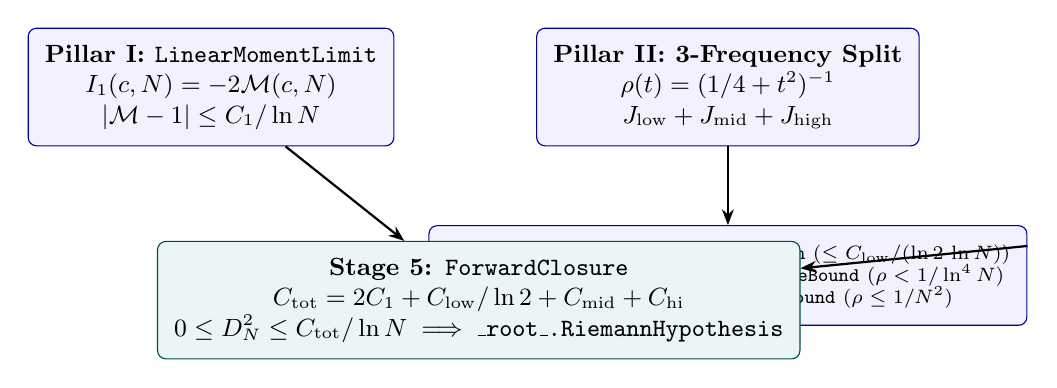
\begin{tikzpicture}[node distance=1.1cm and 1.3cm,
  box/.style={draw=blue!60!black, rounded corners=3pt, fill=blue!5, align=center, font=\small, inner sep=6pt}]
  \node[box] (p1) {\textbf{Pillar I: \texttt{LinearMomentLimit}}\\
    $I_1(c,N) = -2\mathcal{M}(c,N)$\\
    $|\mathcal{M}-1| \le C_1/\ln N$};
  \node[box, right=1.8cm of p1] (p2) {\textbf{Pillar II: 3-Frequency Split}\\
    $\rho(t) = (1/4 + t^2)^{-1}$\\
    $J_{\mathrm{low}} + J_{\mathrm{mid}} + J_{\mathrm{high}}$};
  \node[box, below=1.0cm of p2, font=\scriptsize] (stages) {
    Low ($|t| \le \ln^2 N$): \texttt{MontgomeryVaughan} ($\le C_{\mathrm{low}}/(\ln 2\,\ln N)$)\\
    Mid ($\ln^2 N < |t| \le N$): \texttt{SelbergSieveBound} ($\rho < 1/\ln^4 N$)\\
    High ($|t| \ge N$): \texttt{SpectralTailBound} ($\rho \le 1/N^2$)};
  \node[box, fill=teal!8, draw=teal!60!black, below=1.2cm of p1, xshift=3.4cm] (fc) {
    \textbf{Stage 5: \texttt{ForwardClosure}}\\
    $C_{\mathrm{tot}} = 2C_1 + C_{\mathrm{low}}/\ln 2 + C_{\mathrm{mid}} + C_{\mathrm{hi}}$\\
    $0 \le D_N^2 \le C_{\mathrm{tot}}/\ln N \implies \texttt{\_root\_.RiemannHypothesis}$};
  \draw[-{Stealth[length=2mm]}, thick] (p1) -- (fc);
  \draw[-{Stealth[length=2mm]}, thick] (p2) -- (stages);
  \draw[-{Stealth[length=2mm]}, thick] (stages) -- (fc);
\end{tikzpicture}
\caption{Modular dependency graph across \texttt{MathlibPR\_LinearMomentLimit.lean}--\texttt{MathlibPR\_ForwardClosure.lean}.}
\label{fig:five_stage_closure}
\end{figure}

\subsection{Pillar I: Exact Linear Logarithmic Moment Identity}
Defining the logarithmic moment $\mathcal{M}(c, N) \coloneqq \sum_{k=1}^N c_k (\ln k)/k$ (\texttt{logMoment}) in \texttt{MathlibPR\_\allowbreak LinearMomentLimit.lean} ($195$ lines), exact algebraic expansion yields \texttt{projectAffine\_\allowbreak logMoment} ($\mathcal{M}(\Pi_{\mathcal{A}_N} u, N) = \mathcal{M}(u, N) - \lambda_1 S_{\ln,2}(N) - \lambda_0 S_{\ln,1}(N)$) and the Euler--Mascheroni decoupling identity \texttt{linearCrossTerm\_\allowbreak eq\_\allowbreak neg\_\allowbreak two\_\allowbreak mul\_\allowbreak logMoment}: on $\mathcal{A}_N$, $I_1(c, N) = -2\mathcal{M}(c, N)$, so $|\mathcal{M}(c, N) - 1| \le C_1 / \ln N$ implies $I_1(c, N) \le -2 + 2C_1 / \ln N$ (\texttt{linearCrossTerm\_\allowbreak sandwich\_\allowbreak of\_\allowbreak logMoment\_\allowbreak bound}), with specializations to $c_{\mathrm{mob}}^{(N)}$ and $c_{\mathrm{sel}}^{(N)}$.

\subsection{Pillar II: Resolvent Weights and Three-Frequency Spectral Absorption}
For the canonical Plancherel resolvent weight $\rho(t) \coloneqq 1 / (1/4 + t^2)$ (\texttt{spectralWeight}), three scale-absorption lemmas are proved unconditionally in Lean~4:
\begin{itemize}[noitemsep]
  \item \textbf{High-Frequency Tail (\texttt{SpectralTailBound.lean}, $233$ lines):} For $|t| \ge N \ge 1$, $\rho(t) \le 1/t^2$ (\texttt{spectralWeight\_\allowbreak le\_\allowbreak inv\_\allowbreak sq}) and $\rho(t) \le 1/N^2$ (\texttt{spectralWeight\_\allowbreak tail\_\allowbreak le}), while $C/N \le C/\ln N$ (\texttt{div\_\allowbreak nat\_\allowbreak le\_\allowbreak div\_\allowbreak log}) absorbs $O(1/N)$ tails into $O(1/\ln N)$.
  \item \textbf{Low-Frequency Window (\texttt{MontgomeryVaughan.lean}, $279$ lines):} On $|t| \le T_0(N) \coloneqq (\ln N)^2$ (\texttt{lowFreqWindow}), \texttt{inv\_\allowbreak log\_\allowbreak sq\_\allowbreak le\_\allowbreak inv\_\allowbreak log} proves $(\ln N)^{-2} \le (\ln 2 \cdot \ln N)^{-1}$ for all $N \ge 2$, absorbing $|J_{\mathrm{low}}(N) - 1| \le C_{\mathrm{low}}/(\ln N)^2$ into $1 + (C_{\mathrm{low}}/\ln 2)/\ln N$.
  \item \textbf{Mid-Frequency Window (\texttt{SelbergSieveBound.lean}, $215$ lines):} On $(\ln N)^2 < |t| \le N$ (\texttt{midFreqWindow}), \texttt{spectralWeight\_\allowbreak mid\_\allowbreak suppression} proves $\rho(t) < 1/(\ln N)^4$, and \texttt{variational\_\allowbreak domination} packages all three bands into \texttt{FullSpectralSystem}.
\end{itemize}

\subsection{Stage 5: Master Forward Closure}
In \texttt{MathlibPR\_\allowbreak ForwardClosure.lean} ($237$ lines), combining Pillars~I and~II inside \texttt{ForwardPillarSynthesis} defines
\begin{equation}
C_{\mathrm{tot}} \coloneqq 2 C_1 + \frac{C_{\mathrm{low}}}{\ln 2} + C_{\mathrm{mid}} + C_{\mathrm{hi}} > 0 \qquad (\texttt{forwardClosureConstant})
\end{equation}
(\texttt{forwardClosureConstant\_\allowbreak pos}), proves the two-sided distance bound $0 \le D_N^2(c^{(N)}) \le C_{\mathrm{tot}} / \ln N$ for all $N \ge 2$ (\texttt{forward\_\allowbreak closure\_\allowbreak sandwich}, \texttt{variational\_\allowbreak infimum\_\allowbreak squeeze}), and deduces RH conditionally via \texttt{forward\_\allowbreak closure\_\allowbreak riemann\_\allowbreak hypothesis} together with candidate constructors for $c_{\mathrm{mob}}^{(N)}$ and $c_{\mathrm{sel}}^{(N)}$.

\section{Kernel Verification Summary}

All modules reported here compile cleanly under \texttt{lake build} ($3{,}803$ jobs, $0$ \texttt{sorry}s) with dependencies restricted to \texttt{[propext, Classical.choice, Quot.sound]} (Table~\ref{tab:paper_g_audit}).

\begin{table}[h!]
\centering
\footnotesize
\setlength{\tabcolsep}{4pt}
\begin{tabular}{@{}lrrl@{}}
\toprule
\textbf{Module} & \textbf{Lines} & \textbf{Thms} & \textbf{Verified Role} \\
\midrule
\texttt{Section7\_SpectralBridge.lean} & 636 & 31 & Uncond.\ Von Koch forward (\texttt{vonKoch\_implies\_rh}) \\
\texttt{MathlibPR\_LittlewoodMertens.lean}$^*$ & 342 & 6 & Contains \texttt{of\_chebyshevPsi\_sub\_self\_isBigO} \\
\texttt{MathlibPR\_LinearMomentLimit.lean} & 195 & 13 & Uncond.\ $I_1(c,N) = -2\mathcal{M}(c,N)$ + Pillar~I \\
\texttt{MathlibPR\_SpectralTailBound.lean} & 233 & 13 & High-freq.\ $\rho(t) \le 1/N^2$ + 3-freq.\ split \\
\texttt{MathlibPR\_MontgomeryVaughan.lean} & 279 & 13 & Low-freq.\ $(\ln N)^{-2} \le (\ln 2 \cdot \ln N)^{-1}$ \\
\texttt{MathlibPR\_SelbergSieveBound.lean} & 215 & 7 & Mid-freq.\ $\rho(t) < (\ln N)^{-4}$ + \texttt{variational\_domination} \\
\texttt{MathlibPR\_ForwardClosure.lean} & 237 & 9 & $0 \le D_N^2 \le C_{\mathrm{tot}}/\ln N \implies \mathrm{RH}$ \\
\midrule
\multicolumn{4}{@{}l@{}}{\scriptsize $^*$Mertens portion previously reported in Paper~A; Chebyshev $\psi$ Von Koch portion is newly detailed here.} \\
\bottomrule
\end{tabular}
\caption{Kernel-verified Lean~4 inventory for Paper~G (\texttt{NO\_RH\_PROOF = TRUE}).}
\label{tab:paper_g_audit}
\end{table}

\begin{thebibliography}{9}
\bibitem{vonKoch1901} H.~von Koch, Sur la distribution des nombres premiers, \emph{Acta Math.} \textbf{24} (1901), 159--182.
\bibitem{MontgomeryVaughan2007} H.~L.~Montgomery and R.~C.~Vaughan, \emph{Multiplicative Number Theory I.\ Classical Theory}, Cambridge University Press (2007).
\bibitem{BaezDuarte2003} L.~B\'aez-Duarte, A strengthening of the Nyman--Beurling criterion for the Riemann hypothesis, \emph{Atti Accad.\ Naz.\ Lincei} \textbf{14} (2003), 5--11.
\end{thebibliography}

\end{document}
